\section{Underwater landing vehicle}

The design of an underwater vehicle was made after taking into consideration essential hardware for landing on the seafloor. In this work, we propose the developed of an underwater vehicle with negative buoyancy for landing. The negative buoyancy allows the AUV to land with minimum use of vertical thrust and remain stationary after landing while making seafloor observations. This also saves power and provides a vibration free environment for sensors. 

%*************************************************************************

\subsection{Vehicle hardware}

 The design features on the vehicle can be seen in the Fig.~\ref{f:mehul2}. Two horizontal thrusters provide surge and heading control while two  thrusters, inclined at $22.5^\circ$ with the vertical, control sway and heave. Independent heave, surge, sway and heading control allows the vehicle to perform slow speed manoeuvres and hover when necessary. The inclined thrusters also direct the thrust away from the area directly below the vehicle minimizing the disturbance of sand and sediments during landing. 

\begin{figure}[!ht]
\centering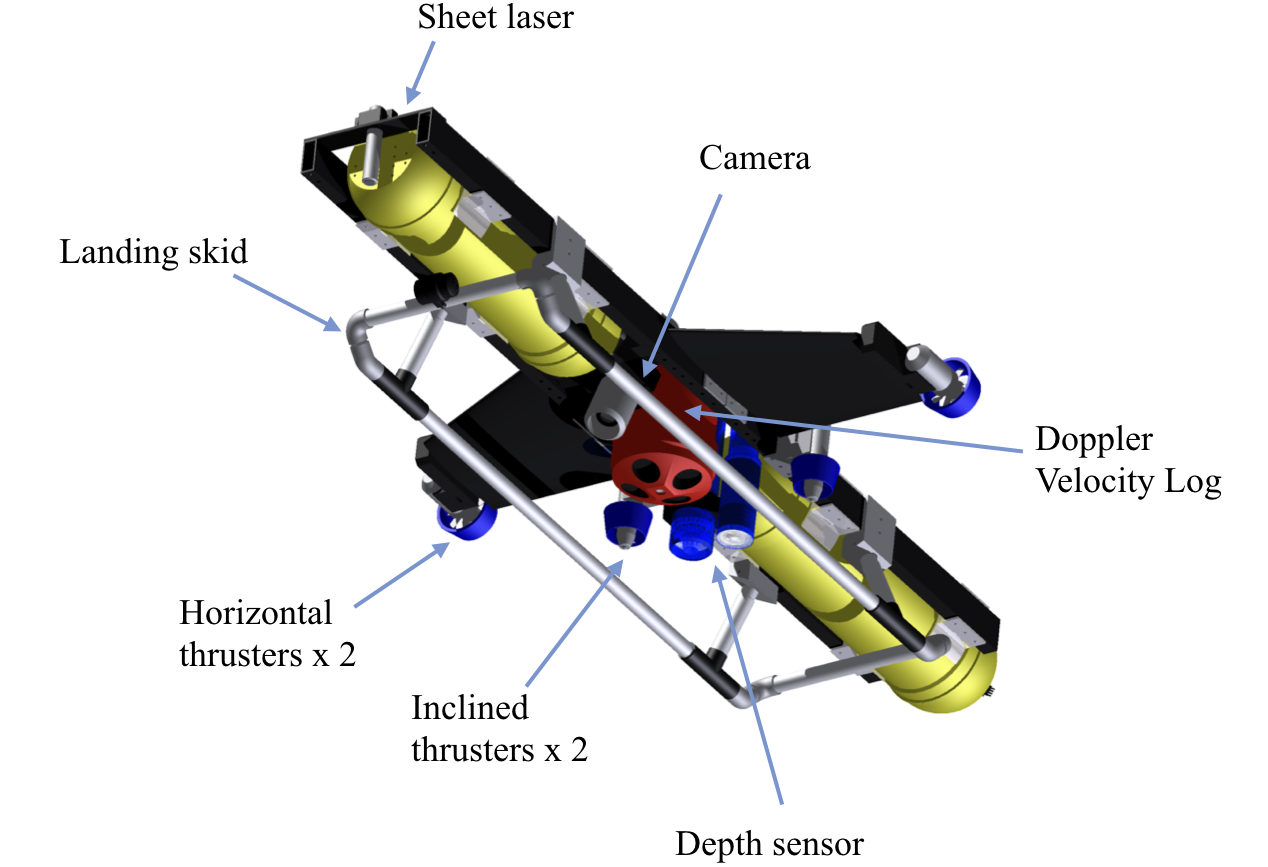
\includegraphics[width=4.7in]{./images/mehul2.png}
\caption{Hardware features on the the underwater vehicle}
\label{f:mehul2}
\end{figure}

The vehicle is designed to be negatively buoyant for landing. Although variable buoyancy engines are available \cite{Zhao2008}, for our vehicle, negative buoyancy was obtained using fixed weights. A NACA$651412$ wing profile is used to offset the negative buoyancy by generating lift during forward motion at zero angle of attack. A nylon landing skid provides stable footing and protects sensors under the vehicle. Navigation is performed using dead reckoning by integrating the velocity obtained from a Doppler Velocity Log (DVL) and orientation with a pressure depth sensor to estimate the state of the vehicle at any moment in time. Although during landing, the vehicle can use altitude measurements from DVL beam range to estimate its distance from the seafloor, these fail to work below $0.3$ m  range. We propose to use record the depth of the vehicle before landing from an altitude of $1$ m and  estimate the depth at the landing point. 

\subsection{High resolution mapping system}
\label{ssec:hres}

A high resolution mapping system ~\cite{Bodenmann2016} using light sectioning is integrated into the vehicle for generating mm-resolution bathymetry. The hardware components of the system can be seen in Fig.~\ref{f:mehul3} and the parameters associated are explained in the Table~\ref{t:table0}. The system uses a sheet laser which projects a laser on the seafloor whose projection is captured by a camera mounted at an angle. The pixels in the image belonging to the laser image are identified and converted to local coordinates using the geometry of the system. These are then converted to earth coordinates using the position of the vehicle. 

\begin{figure}[!ht]
\centering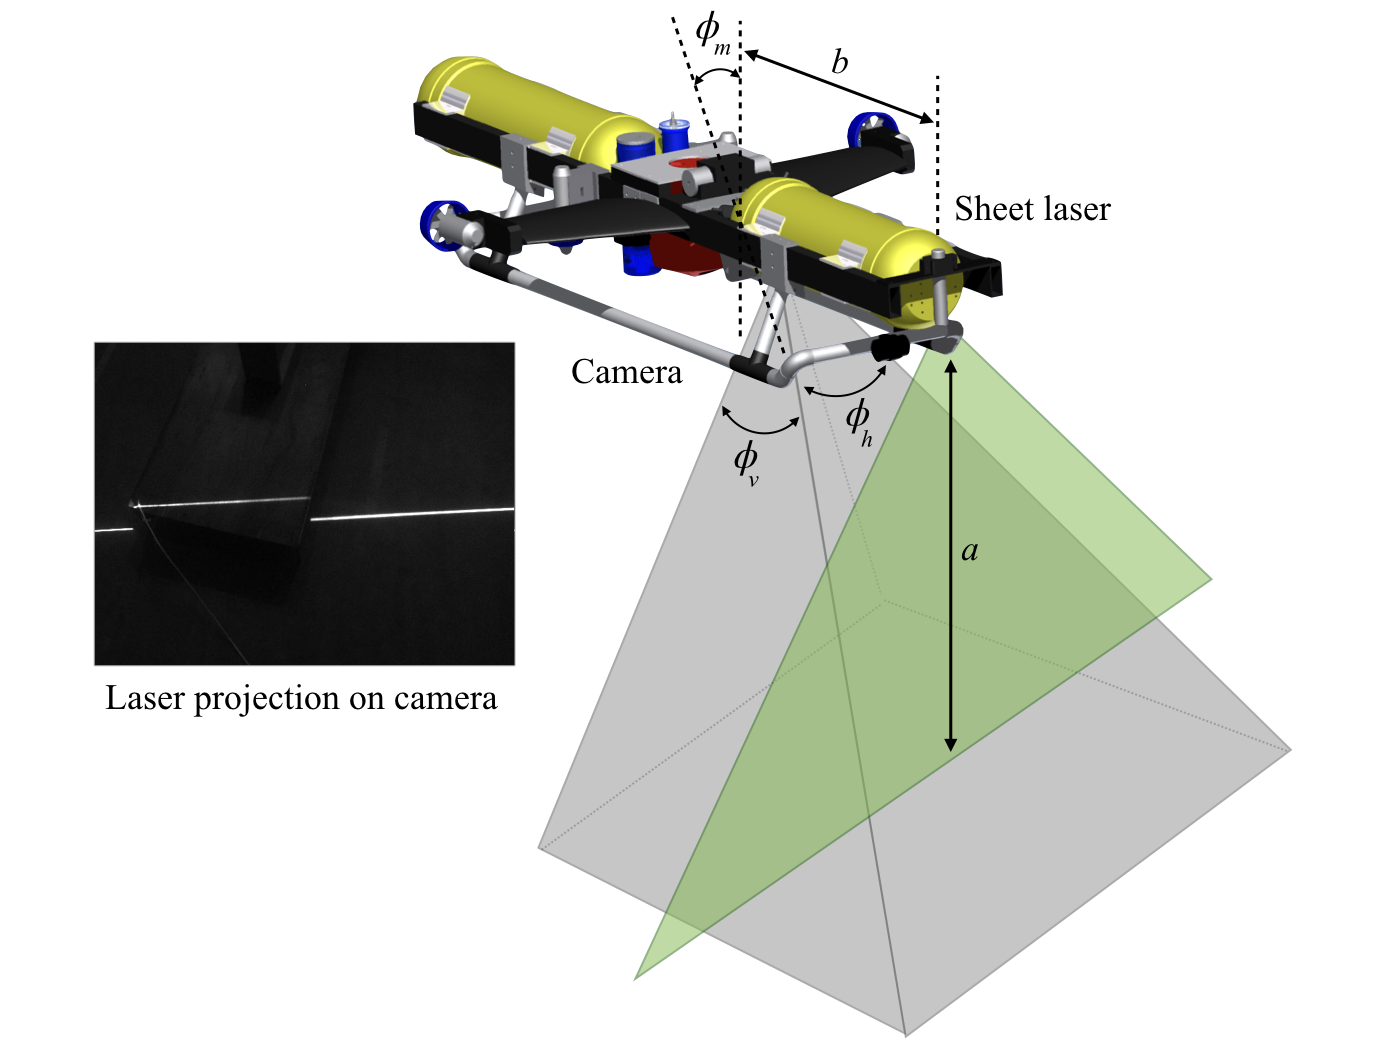
\includegraphics[width=4.7in]{./images/mehul3.png}
\caption{Setup and working of the high resolution mapping system}
\label{f:mehul3}
\end{figure}

\begin{table}[!ht]
\centering
\caption{Parameters of the mapping system}
\begin{tabular}{  |p{6cm}  p{4cm}| }
\hline
\textbf{Property} & \textbf{Value}\\ \hline 
Mapping altitude & $a$\\
Baseline between camera and laser & $b$\\
Vertical mounting angle of camera & $\phi_m$\\
Horizontal opening angle of camera & $\phi_h$\\
Vertical opening angle of camera & $\phi_v$\\
\hline
\end{tabular}
\label{t:table0}
\end{table}

 